\documentclass{subfiles}
\begin{document}
Il filtro gradiente è un filtro digitale che mette in evidenza i contorni di un'immagine, sfruttando il concetto matematico di gradiente.
Per tale filtro l'immagine è considerata come una funzione a due variabili \(I(x,y)\), sulla quale è appunto calcolabile il gradiente.
Si ricorda che il gradiente, da un punto di vista matematico,
\begin{wrapfigure}[15]{r}{0.425\textwidth}
    \centering
    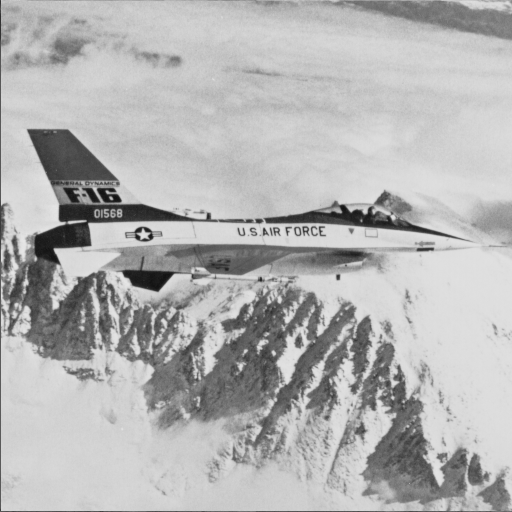
\includegraphics[scale = 0.325]{../Images/Airplane/AirplaneGS.png}
    \caption{AirplaneGS}
    \label{fig:4.8}
\end{wrapfigure}
è definito come
\[
    \grad{I(x,y)} = \left(\pdv{f}{x} i, \pdv{f}{y} j\right)
\]

Dalla definizione continua del rapporto incrementale, si può derivare la definizione discreta delle componenti di \(\grad{I(x, y)}\), la quali risultano essere
\[\begin{aligned}
        \pdv{f}{x} & \approx I(x, y+1) - I(x, y) = \Delta_{x}f = \begin{bmatrix}
                                                                     -1 & 1 \\
                                                                 \end{bmatrix}   \\
        \pdv{f}{y} & \approx I(x + 1, y) - I(x, y) = \Delta_{y}f = \begin{bmatrix}
                                                                       -1 \\
                                                                       1  \\
                                                                   \end{bmatrix}
    \end{aligned}\]

La definizione data risulta sensata dato che, il pixel \(p_{1}\) più prossimo ad un pixel \(p_{0}\) è banalmente quello ad esso adiacente.

Si consideri ora \emph{Figura \ref{fig:4.8}}. Procedendo dunque col calcolare le derivare in ambo le direzioni della stessa,
quel che ne risulta è mostrato in \emph{Figura \ref{fig:4.9}}.
\subfile{../Figure/Figure 4.9 - Derivate di Airplane.tex}
Da questa si evince che calcolare la derivate di un'immagine lungo una direzioni, equivale a mettere in risalto i contorni lungo l'altra.

\begin{Remark*}
    per una questione di visibilità, le derivate di \emph{Figura \ref{fig:4.9}} sono state moltiplicate per un apposita costante,
    mettendo così in risalto contorni che con le derivate originali sarebbero impercettibili.
\end{Remark*}

Essendo il gradiente un vettore, questi ammette modulo e l'orientamento, che si ricordano essere calcolate come
\[
    \norm{\grad{I(x,y)}} = \sqrt{\Delta_{x}^{2}f + \Delta_{y}^{2}f} \quad \text{e} \quad \measuredangle I = \arctan \frac{\Delta_{y}}{\Delta_{x}}
\]

Considerando dunque questi ultimi, è possibile calcolare la norma e l'orientamento di un'immagine.
Partendo dalla norma: essendo questa la radice quadrata della somma dei quadrati
\begin{wrapfigure}[10]{r}{0.425\textwidth}
    \centering
    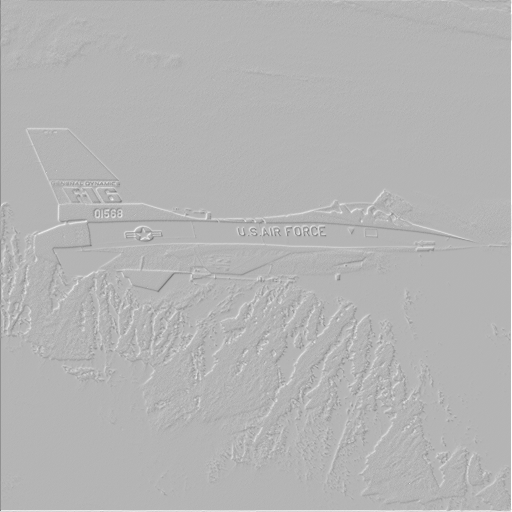
\includegraphics[scale = 0.325]{../Images/Airplane/ModulesAirplane.png}
    \caption{Contorni  omnidirezionali di \emph{Figura \ref{fig:4.9}}}
    \label{fig:4.10}
\end{wrapfigure}
delle derivate, effettuare la norma di un immagine, equivale a mettere in evidenza i contorni della stessa in ogni direzione.
Quanto appena detto è mostrato in \emph{Figura \ref{fig:4.10}} ottenuta come norma di \emph{Figura \ref{fig:4.8}}.

Per quel che concerne i segmenti di codici utilizzati per ricavare le immagini di \emph{Figura \ref{fig:4.9} \emph{e} \ref{fig:4.10}},
questi sono di seguito riportati nel rispettivo ordine.
\begin{center}
    \begin{lstlisting}[language = MATLAB]
        % caricamento di AirplaneGS.png
        dx = conv2(AirplaneGS, [-1, 1], `same');
        figure; imshow(dx, [0, 255]);
    \end{lstlisting}
    \begin{lstlisting}[language = MATLAB]
        % caricamento di AirplaneGS.png
        dy = conv2(AirplaneGS, [-1; 1], `same');
        figure; imshow(dx, [0, 255]);
    \end{lstlisting}
    \begin{lstlisting}[language = MATLAB]
        % dx e dy sono le immagine sin ora calcolate
        normA = sqrt(dx.^2 + dy.^2);
        figure; imshow(normA, [0, 255]);
    \end{lstlisting}
\end{center}

\begin{Note*}
    l'utilizzo di ``.\textasciicircum '' nei codici di cui sopra, è utilizzato per indicare che il quadrato non è della matrice, ma si tratta di un quadrato punto-punto.
\end{Note*}
\begin{wrapfigure}{l}{0.425\textwidth}
    \centering
    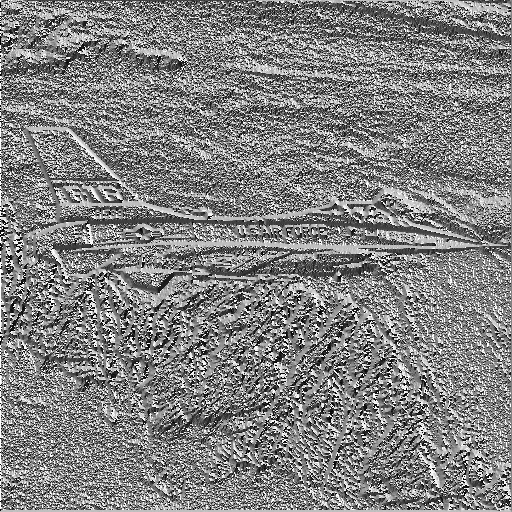
\includegraphics[scale = 0.325]{../Images/Airplane/OrientationAirplane.png}
    \caption{\emph{Figura \ref{fig:4.9}} da un punto di vista dell'orientamento dei moduli del gradiente.}
    \label{fig:4.11}
\end{wrapfigure}
Passando al considerare l'orientamento, questi è ottenuto punto per punto come arcotangente del rapporto delle due derivate,
volendo dunque osservare a cosa ciò equivalga, eseguendo l'opportuno codice MATLAB, a seguire, quel che si ottiene è mostrato in \emph{Figura \ref{fig:4.11}}.
\begin{center}
    \begin{lstlisting}[language = MATLAB]
            % dx e dy sono le immagine sin ora calcolate
            orientation = atan2(double(dx), double(dy));
            figure; imshow(orientation, [-pi, pi]);
        \end{lstlisting}
\end{center}
\end{document}